\documentclass[article, a5paper]{memoir}

\newcommand{\Version}{Version 1.6}

\let\footruleskip\undefined\usepackage{fancyhdr}% http://ctan.org/pkg/fancyhdr

\usepackage{pgfpages}
\pgfpagesuselayout{resize to}[a4paper]

% Swedish.
\usepackage[utf8]{inputenc}
\usepackage[T1]{fontenc}
%\usepackage[swedish]{babel}
\usepackage{microtype}

%%% FONT PACKAGES
%\usepackage[sc]{mathpazo}
%\usepackage[varg]{txfonts}
%\usepackage{times}
%\usepackage{tgtermes}% clone of times
%\usepackage[sfdefault,condensed]{cabin}
\usepackage{PTSansNarrow}\renewcommand*\familydefault{\sfdefault}
%\usepackage{tgcursor}
\usepackage[scaled=0.85]{beramono} % inconsolata or beramono ???
%\usepackage{fouriernc} % serif: new century schoolbook
%\usepackage{avant}     % sans serif: Avant Garde


% Typeblock size, margins.
\settypeblocksize{190mm}{127mm}{*}
\setlrmargins{10.5mm}{*}{*}
\setulmargins{10.0mm}{*}{*}
\setheadfoot{0.1pt}{0.1pt}
\checkandfixthelayout

\usepackage{multicol} \setlength{\columnsep}{5mm}
\usepackage{xcolor}
\usepackage{array}

\definecolor{commentgreen}{rgb}{0,0.4,0}
\definecolor{grammarcolor}{rgb}{0.3,0.6,0.1}
\definecolor{mylinkcolor}{rgb}{0,0.1,0.5}
\definecolor{myemphcolor}{rgb}{0,0.4,0.1}
\definecolor{myalertcolor}{rgb}{0.4,0.1,0}
\definecolor{eclipsepurple}{rgb}{0.5,0,0.25}
\definecolor{eclipseblue}{rgb}{0.16,0,1.0}
\definecolor{eclipsegreen}{rgb}{0,0.5,0}


\newcommand{\OptL}{\textbf{\textcolor{grammarcolor}{~[~}}}
\newcommand{\OptR}{\textbf{\textcolor{grammarcolor}{~]~}}}
\newcommand{\RepL}{\textbf{\textcolor{grammarcolor}{~(~}}}
\newcommand{\RepR}{\textbf{\textcolor{grammarcolor}{~)~}}}
\newcommand{\Or}{\textbf{\textcolor{grammarcolor}{~|~}}}


%---------------------------------------------------------------

\newcommand{\LangColor}{red}

\setlength{\parindent}{0pt}
\raggedright
\raggedbottom
\linespread{0.90}\selectfont
\pagestyle{empty}

\newcommand{\mc}[1]{\multicolumn{2}{l}{\hspace{-0.65em}\parbox[t]{102mm}{\small #1}}}

\newcommand{\ind}{\hspace*{1.5em}}

\newcommand{\head}[1]{{\bfseries {\color{\LangColor}{#1}}\par\vspace{1mm}\hrule\vspace{-2mm}}}

\newenvironment{etab}%
{\begin{ctabular}{@{}>{\raggedright\small}p{25mm} @{}>{\raggedright\small}p{45mm} @{}>{\raggedright\arraybackslash\small}p{57mm}}}
{\end{ctabular}}%


\newcommand{\secend}{\\[1mm]}
\newcommand{\subsecend}{\\ \\[-2mm]}
\renewcommand{\arraystretch}{0.9}

% -----------
\usepackage{tikz}
\usetikzlibrary{calc}
\usetikzlibrary{shapes.geometric, shapes.symbols, arrows, matrix, shapes, positioning}
%https://www.sharelatex.com/blog/2013/08/29/tikz-series-pt3.html
\tikzstyle{startstop} = [rectangle, rounded corners, minimum width=3cm, minimum height=1cm,text centered, draw=black, fill=red!30]
\tikzstyle{io} = [trapezium, trapezium left angle=70, trapezium right angle=110, minimum width=1cm, minimum height=1cm, text=white, text centered, draw=black, fill=blue!50!violet]
\tikzstyle{process} = [rectangle, minimum width=3cm, minimum height=1cm, text=white, text centered, draw=black, fill=red!50!black]
\tikzstyle{decision} = [diamond, minimum width=3cm, minimum height=1cm, text centered, draw=black, fill=green!30]
\tikzstyle{arrow} = [thick,->,>=stealth]
%UML definitions
\tikzstyle{umlclass}=[rectangle, draw=black,  thick, anchor=north, text width=3cm, rectangle split, rectangle split parts = 3]
\tikzstyle{umlarrow}=[->, >=open triangle 90, thick]

%%%%%%%%%%%%%%%%%%%%%%%%%%%%
%%% lingstings specifics:
\usepackage{listings}
\usepackage{upquote} %http://tex.stackexchange.com/questions/145416/how-to-have-straight-single-quotes-in-lstlistings
\lstdefinelanguage{Scala}{
  morekeywords={abstract,case,catch,class,def,%
    do,else,extends,false,final,finally,%
    for,forSome,if,implicit,import,lazy,match,%
    new,null,object,override,package,%
    private,protected,return,sealed,%
    super,this,throw,trait,true,try,%
    type,val,var,while,with,yield},
  otherkeywords={=>,<-,<\%,<:,>:,@},
  sensitive=true,
  morecomment=[l]{//},
  morecomment=[n]{/*}{*/},
  morestring=[b]",
  morestring=[b]',
  morestring=[b]"""
}


\lstset{
    language=Scala,
    tabsize=2,
    basicstyle=\ttfamily\selectfont,
    keywordstyle=\bfseries\textcolor{eclipsepurple},
    commentstyle=\textcolor{commentgreen},
    numberstyle={\footnotesize},
    numbers=none,
    %backgroundcolor=\textcolor{gray!15},
    frame=none,
    rulecolor=\color{black!25},
    %title={\footnotesize\lstname},
    breaklines=false,
    breakatwhitespace=false,
    framextopmargin=2pt,
    framexbottommargin=2pt,
    showstringspaces=false,
    columns=fullflexible,keepspaces
}
\lstset{literate=%
{Å}{{\AA}}1
{Ä}{{\"A}}1
{Ö}{{\"O}}1
{Ü}{{\"U}}1
{ß}{{\ss}}1
{ü}{{\"u}}1
{å}{{\aa}}1
{ä}{{\"a}}1
{ö}{{\"o}}1
{æ}{{\ae}}1
{ø}{{\o}}1
{Æ}{{\AE}}1
{Ø}{{\O}}1
{`}{{\`{}}}1
{─}{{\textemdash}}1
{└}{{|}}1
{├}{{|}}1
{│}{{|}}1
}

\newcommand{\code}{\lstinline[basicstyle=\ttfamily]}
\newcommand{\jcode}{\lstinline[basicstyle=\ttfamily,language=Java]}

\lstnewenvironment{Code}[1][]{%
    \lstset{basicstyle=\ttfamily\fontsize{9}{11}\selectfont,#1}%
}{}

%*****************************************************************



\newcommand{\LangRect}[5]{\tikz[overlay, remember picture,inner sep=7pt,minimum height=0.65cm] \node[fill=#2,text=white,rotate=90] at #4 (name) {\large\normalfont\textbf{#1} ~~{\small \thepage(#5)}}; }  

\newcommand{\LangRectOdd}[4]{\LangRect{#1}{#2}{#3}{($(current page.north east)-(0.35,#3)$)}{#4}}  
\newcommand{\LangRectEven}[4]{\LangRect{#1}{#2}{#3}{($(current page.north west)-(-0.35,#3)$)}{#4}}  
    

\newcommand{\LangMarker}[3]{%param 1 = language, param 2 = offset from top
%\fancyhead{} % clear all header fields
\fancyfoot{} % clear all footer fields
%\fancyfoot[RO]{\thepage}
%\fancyfoot[LE]{\thepage}
\fancyhead{
\ifodd\thepage\LangRectOdd{#1}{\LangColor}{#2}{#3}
\else\LangRectEven{#1}{\LangColor}{#2}{#3}
\fi 
}
\renewcommand{\headrulewidth}{0pt}
\renewcommand{\footrulewidth}{0pt}
\pagestyle{fancy}
}

\newcommand{\Newline}{\vspace{\baselineskip}}

\newcommand{\LangTitle}[1]{{\centering \Huge{\bfseries\sffamily \color{\LangColor}{#1}}\par}}

\newcommand{\Comment}[1]{{\color{commentgreen}{#1}}}

\begin{document}

\LangMarker{Scala}{1.5cm}{8}
\LangTitle{Scala Quick Ref @ Lund University}
{\centering https://github.com/lunduniversity/introprog/tree/master/quickref \\
{\small \Version. License: CC-BY-SA, \textcopyright~Dept. of Computer Science, Lund University.}\\
{\small Pull requests welcome! Contact: bjorn.regnell@cs.lth.se}
\par}

%%%%%%%%%%%%%%%%%%%%%%%%%%%%%%%%%%%%%%%%%%%%%%%%%%%%%%%%%%%%%%
\vspace{0.5em}
\head{Top-level definitions} \vspace{0.75em}
\hspace{0.32em}\begin{minipage}{0.52\linewidth}%
\begin{Code}[frame=single] %[frame=single]  [frame=none]
// in file: hello.scala
package x.y.z
object HelloWorld {
  def main(args: Array[String]): Unit = { 
    println("Hi " + args.mkString(" ")) 
  }
}
\end{Code}%
\end{minipage}%
\hfill\begin{minipage}{0.45\linewidth}
\raggedright{\small
A compilation unit (here hello.scala) consists of a sequence of packagings, import clauses, and class and object definitions, which may be preceded by a package clause, e.g.: \code|package x.y.z |that places the compiled file HelloWorld.class in directory x/y/z/

\begin{tabular}{@{}r @{\hspace{0.5em}}l} \\[-0.5em]
\textbf{Compile}:  & \verb|scalac hello.scala| \\
\textbf{Run}:  &  \verb|scala x.y.z.HelloWorld args| \\[0.1em]
&Execution starts in method main.
\end{tabular}%
}%
\end{minipage} 
%%%%%%%%%%%%%%%%%%%%%%%%%%%%%%%%%%%%%%%%%%%%%%%%%%%%%%%%%%%%%%


%%%%%%%%%%%%%%%%%%%%%%%%%%%%%%%%%%%%%%%%%%%%%%%%%%%%%%%%%%%%%%
\vspace{0.1em}
\head{Definitions and declarations}\Newline
{\small\renewcommand{\arraystretch}{0.95}
A \textbf{definition} binds a name to a value/implementation, while a \textbf{declaration} just introduces a name (and type) of an abstract member. Below \code|defsAndDecl| denotes a list of definitions and/or declarations.   
\newcommand{\MoveUp}{\\[-0.9em]}
\newcommand{\FirstColWidth}{0.65cm}
\begin{tabular}{@{}p{\FirstColWidth} l l}\\
%\textbf{What} & \textbf{Example} & \textbf{Exlpanation} \\ \hline \\[-0.5em]
Variable 
& \code|val x = expr|  & \Comment{Variable x is assigned to expr. A \textbf{val} can only be \textbf{assigned once}.}\\
& \code|val x: Int = 0|  & \Comment{Explicit type annotation,  expr: SomeType allowed after any expr.}\\ 
& \code|var x = expr|  & \Comment{Variable x is assigned to expr. A \textbf{var} can be \textbf{re-assigned}.} \\
& \code|val x, y = expr| & \Comment{Multiple initialisations, x and y is initialised to the same value.}\\
& \code|val (x, y) = (e1, e2)| & \Comment{Tuple pattern initialisation, x is assigned to e1 and y to e2.}\\
& \multicolumn{2}{l}{\code|val Seq(x, y) = Seq(e1, e2)|  \Comment{Sequence pattern initialisation, x is assigned to e1 and y to e2.}}\\
& \code|val x: Int = _| & \Comment{Initialized to default value, 0 for number types, null for AnyRef types.}\\
\end{tabular}

\begin{tabular}{@{}p{\FirstColWidth} l l}\MoveUp
Function
& \code|def f(a: Int, b: Int): Int = a + b| & \Comment{Function f of type (Int, Int) => Int}\\
& \code|def f(a: Int = 0, b: Int = 0): Int = a + b| & \Comment{Default arguments used if args omitted, f().}\\

&  \code|f(b = 1, a = 3)| & \Comment{{\hspace{-0.25em} Named arguments can be used in any order.}}\\
& \code|def add(a: Int)(b: Int): Int = a + b| & \Comment{Multiple parameter lists, apply: add(1)(2)} \\

& \code|(a: Int, b: Int) => a + b| & \Comment{Anonymous function value, ''lambda''.}\\
& \code|val g: (Int, Int) => Int = (a, b) => a + b| & \Comment{Types can be omitted in lambda if inferable.}\\

& \multicolumn{2}{l}{\code|f _| \hspace{4.8em} \Comment{Replacing a parameter list with a space and underscore gives the function itself as a value.}}\\

& \multicolumn{2}{l}{\code|val inc = add(1) _ | \hspace{-4.25em} \Comment{\hspace{6em} Partially applied function add(1) of add above, where inc is of type Int => Int}}\\

& \multicolumn{2}{l}{\code|def addAll(xs: Int*) = xs.sum |  \Comment{\hspace{0.42em} Repeated parameters: addAll(1,2,3) or addAll(Seq(1,2,3): \_*) }}\\

& \multicolumn{2}{l}{\code|def twice(block: => Unit) = \{ block; block \}| \Comment{\hspace{0.5em} Call-by-name argument evaluated later.}}\\
\end{tabular}

\begin{tabular}{@{}p{\FirstColWidth} l l}\MoveUp
Object
& \code|object Name { defsAndDecl } | \Comment{Singleton object auto-allocated when referenced the first time.}
\end{tabular}

\begin{tabular}{@{}p{\FirstColWidth} l l}\MoveUp
Class
& \code|class C(parameters) { defsAndDecl }| & \hspace{-3.2em}\Comment{A template for objects, which are allocated with \textbf{new}.} \\
& \code|case class C(parameters) { defsAndDecl }| & \Comment{Case class parameters become val members,} \\
& \multicolumn{2}{l}{\Comment{other case class goodies: equals, copy, hashcode, unapply, nice toString, companion object with apply factory.}}\\
\end{tabular}

\begin{tabular}{@{}p{\FirstColWidth} l l}\MoveUp
Trait
& \code|trait T { defsAndDecl }| & \hspace{-1.1em}\Comment{A trait is like an abstract class, but can be mixed in; can't have parameters.}\\ 
& \code|class C extends D with T| & \hspace{-0.9em}\Comment{A class can only \textbf{extend} one class but mix in many traits using \textbf{with}.}\\
\end{tabular}

\begin{tabular}{@{}p{\FirstColWidth} l l}\MoveUp
Type
& \code|type A = typeDef | & \Comment{Defines an alias A for the type in typeDef. Abstract if no typeDef.}
\end{tabular}

\begin{tabular}{@{}p{\FirstColWidth} l @{}l}\MoveUp
Import
& \code|import path.to.module.name | & \Comment{Makes name directly visible. Underscore imports all.}\\
& \code|import path.to.{a, b => x, c => _} | & \Comment{Import several names, b renamed to x, c not imported.}\\
\end{tabular}
}% end small

\vspace{0.6em}
{\small
\begin{tabular}{@{}l @{}l l}
\textbf{Modifier} & \textbf{applies to} & \textbf{semantics}\\ \hline \\[-0.7em]
\code|private[this] | & definitions, declarations & \Comment{Restricts access to this instance only; also private[p] for package p.} \\
\code|private| & definitions, declarations & \Comment{Restricts access to directly enclosing class and its companion.}\\
\code|protected| & definitions& \Comment{Restricts access to subtypes and companion.}\\
\code|override| & definitions, declarations & \Comment{Mandatory if overriding  a concrete definition in a parent class.}\\
\code|abstract| & class definitions & \Comment{Abstract classes cannot be instantiated (redundant for traits).}\\
\code|final| &  definitions & \Comment{Final members cannot be overridden, final classes cannot be extended.}\\
\code|lazy| & val definitions & \Comment{Delays initialization of val, initialized when first referenced.}\\
\code|sealed| & class definitions & \Comment{Restricts direct inheritance to classes in the same source file.}
\\
\end{tabular}
}

%%%%%%%%%%%%%%%%%%%%%%%%%%%%%%%%%%%%%%%%%%%%%%%%%%%%%%%%%%%%%%
\vspace{-1.5em}\head{Special methods}\Newline
{\small
\begin{tabular}{@{}l @{}l}
\code|class A(initX: Int = 0) {| & \Comment{\textbf{primary constructor}: new A(1) or using default arg: new A()} \\
\code|  private var _x = initX| & \Comment{private member only visible in A and its companion} \\
\code|  def x: Int = _x| & \Comment{\textbf{getter} for private field \_x (name chosen to avoid clash with x)} \\
\code|  def x_=(i: Int): Unit = { _x = i } | & \Comment{special \textbf{setter} assignment syntax: val a = new A(1); a.x = 2} \\
\code|  | & \Comment{} \\
\code|}| & \\
\code|object A {| & \Comment{\textbf{companion object} if same name and in same code file} \\
\code|  def apply(i: Int = 0) = new A(i) |  & \Comment{\textbf{factory method} makes new unnecessary:  A.apply(1), A(1), A()} \\
\code|  val a = A(1)._x | & \Comment{private members can be accessed in companion} \\
\code|}|  \\
\end{tabular}


\vspace{0.5em}
Getters and setters above are auto-generated by \textbf{var} in primary constructor:
 {\hfill\code|class A(var x: Int = 0)|}\\
With \textbf{val} in primary constructor only getter, no setter, is generated:
 {\hfill\code|class A(val x: Int = 0)|} \\
\textbf{Private constructor} e.g. to enforce use of factory in companion only: 
{\hfill\code|class A private (var x: Int = 0)|} \\
Instead of default arguments, an \textbf{auxiliary constructor} can be defined (less common): {\hfill\code|def this() = this(0)|}

\vspace{-0.2em}\hspace{0.32em}\begin{minipage}{0.65\linewidth}%
{\small\begin{Code}[frame=none] %[frame=single]  [frame=none]
class IntVec(private val xs: Array[Int]) {
  def update(i: Int, x: Int): Unit = { xs(i) = x }
  def apply(i: Int): Int = xs(i)
}
\end{Code}%
}%
\end{minipage}%
\hfill\begin{minipage}{0.32\linewidth}
\vspace{-0.5em}\raggedright{\small
Special syntax for \textbf{update} and \textbf{apply}: \\
v(0) = 0~\Comment{expanded to} v.update(0,0)\\
v(0)\hspace{1.5em}\Comment{expanded to} v.apply(0)\\
\Comment{where} val v = new IntVec(Array(1,2,3)) \\

}%
\end{minipage}

}
%%%%%%%%%%%%%%%%%%%%%%%%%%%%%%%%%%%%%%%%%%%%%%%%%%%%%%%%%%%%%%




%%%%%%%%%%%%%%%%%%%%%%%%%%%%%%%%%%%%%%%%%%%%%%%%%%%%%%%%%%%%%%
\Newline\head{Expressions}\Newline
{\small\renewcommand{\arraystretch}{1.05}
\begin{tabular}{@{}l @{\hspace{0.9em}}l @{\hspace{0.2em}}l}
literals  &  \code|0 0L 0.0 "0" '0' true false|   & \Comment{Basic types e.g. Int, Long, Double, String, Char, Boolean} \\

block     &  \code|{ expr1; ...; exprN } |         &  \Comment{The value of a block is the value of its last expression}   \\
if        &  \code|if (cond) expr1 else expr2 |  & \Comment{Value is expr1 if cond is true, expr2 if false (else is optional)} \\
match     &  \code|expr match caseClauses |  &  \Comment{Matches expr against each case clause, see pattern matching. } \\

for       &  \code|for (x <- xs) expr |          &   \Comment{Loop for each x in xs, x visible in expr, type Unit }  \\
yield     &  \code|for (x <- xs) yield expr|     &   \Comment{Yields a sequence with elems of expr for each x in xs }\\
while     &  \code|while (cond) expr |           &   \Comment{Loop expr while cond is true, type Unit }\\
do while  &  \code|do expr while (cond) |        &   \Comment{Do expr at least once, then loop while cond is true, type Unit}\\
throw     &  \code|throw new Exception("Bang!") |  &  \Comment{Throws an exception that halts execution if not in try catch } \\
try       &  \code|try expr catch pf |           & \Comment{Evaluate partial function pf if exception in expr, where pf e.g.: } \\
          & & \code|{case e: Exception => someBackupValue}| \\ 


\end{tabular}

\vspace{0.25em}\renewcommand{\arraystretch}{1.05}
\begin{tabular}{@{}l @{\hspace{-1.6em}}r @{\hspace{0.6em}}l | r l}

Evaluation order   & \code|(1 + 2) * 3| & \Comment{parenthesis control order} & \multicolumn{2}{l}{\hspace{-0.2em}\textbf{Precedence} of operators beginning with:}\\ 

Method application & \code|1.+(2)|  &  \Comment{call method + on object 1} & all letters & \textbf{lowest}\\ 

Operator notation  & \code|1 + 2|  &   \Comment{same as 1.+(2)} & \code+|+ \\

Conjunction  & \code|c1 && c2|  &  \Comment{true if both c1 \textbf{and} c2 true}  & \code|^|  \\
Disjunction  & \code+c1 || c2+  &  \Comment{true if c1 \textbf{or} c2 true}  & \code|&|  \\
Negation  & \code|!c|          &  \Comment{logical \textbf{not}, false if c is true}  & \code|=  !| \\

Function application  & \code|f(1, 2, 3)|  &   \Comment{same as f.apply(1,2,3)} & \code|<  >|\\

Function literal  & \code|x => x + 1|  &   \Comment{anonymous function, ''lambda''} & \code|:|\\

Object creation  & \code|new C(1,2)|  &   \Comment{from class C with arguments 1,2} & \code|+ -|\\

Self reference  & \code|this|  &  \Comment{refers to the object being defined} & \code|* / %| \\

Supertype reference & \code|super.m|  &  \Comment{refers to member m of supertype} & other special chars & \textbf{highest} \\ %\cline{4-5}
Non-referable reference & \code|null|  &  \Comment{refers to null object of type Null} & \\

Assignment operator & \code|x += 1|  &  \Comment{expanded to x = x + 1}  &  \\
                    & \code|x -= 1|  &  \Comment{works for any op ending with =} & 
                     \multicolumn{2}{l}{\textbf{Integer division and reminder:}}\\


Empty tuple, unit value& \code|()|  &  \Comment{of type Unit, similar to Java void}  & \multicolumn{2}{l}{\code|a / b|  \Comment{~no decimals if a, b Int, Short, Byte }} \\
2-tuple value   & \code|(1, "hello")| &  \Comment{same as new Tuple2(1, "hello")}  & \multicolumn{2}{l}{\code|a \% b|  \Comment{~fulfills: (a / b) * b + (a \% b) == a}} \\
2-tuple type    & \code|(Int, String)| & \Comment{same as Tuple2[Int, String]}  &  \\
                &                      & \Comment{etc. until Tuple22}  &  \\
\end{tabular}
}%end small
%%%%%%%%%%%%%%%%%%%%%%%%%%%%%%%%%%%%%%%%%%%%%%%%%%%%%%%%%%%%%%

%%%%%%%%%%%%%%%%%%%%%%%%%%%%%%%%%%%%%%%%%%%%%%%%%%%%%%%%%%%%%%
\clearpage\vspace*{-2.0em}\head{Pattern matching, type tests and extractors}\vspace{0.5em}

\vspace{0.25em}\renewcommand{\arraystretch}{1.0}
{\small%
\begin{tabular}{@{}l @{\hspace{-7.1em}}r}
\code|expr match { | 
& \Comment{expr is matched against patterns from top until match found, yielding the expression after =>}\\

\code|  case "hello" => expr | 
& \Comment{\textbf{literal pattern} matches any value equal (in terms of ==) to the literal}\\

\code|  case x: C => expr | 
& \Comment{\textbf{typed variable pattern} matches all instances of C, binding variable x to the instance} \\

\code|  case C(x, y, z) => expr | 
& \Comment{\textbf{constructor pattern} matches values of the form C(x, y, z), args bound to x,y,z}\\
\code|  case (x, y, z) => expr  | & \Comment{\textbf{tuple pattern} matches tuple values, alias for constructor pattern Tuple3(x, y, z)}\\

\code|  case x +: xs => expr | 
& \Comment{\textbf{sequence extractor patterns} matches head and tail, also x +: y +: z +: xs etc.} \\ 

\code+  case p1 | ... | pN => expr + 
& \Comment{matches if at least one \textbf{pattern alternative} p1, p2 ... or pN  matches} \\ 

\code|  case x@pattern => expr | 
& \Comment{a \textbf{pattern binder} with the @ sign binds a variable to (part of) a pattern} \\ 


\code|  case x => expr | 
& \Comment{\textbf{untyped variable pattern} matches any value, typical ''catch all'' at bottom: \textbf{\texttt{case \_ =>}}} \\ 

\code|}                         | & \Comment{Pattern matching on direct subtypes of a \textbf{sealed} class is checked for exhaustiveness by the compiler} \\
\end{tabular}
}% small

\vspace{0.5em}{\small Matching with typed variable pattern \code| x match { case a: Int => a; case _ => 0}| is preferred over \\explicit isInstanceOf tests and casts: \code{ if (x.isInstanceOf[Int]) x.asInstanceOf[Int] else 0}}

\vspace{0.25em}{\small The \textbf{unapply} method can be used in \textbf{extractor} pattern matching (to avoid extra class \& instance), e.g.:}

\vspace{-0.5em}%
\begin{minipage}{0.6\linewidth}%
{\small
\begin{Code}
object Host {
  def unapply(s: String): Option[String] = 
    if (!s.startsWith("http://")) None
    else s.stripPrefix("http://").split('/').headOption
}
\end{Code}
}%small
\end{minipage}%
\begin{minipage}{0.4\linewidth}
\vspace{-0.2em}{\hfill\raggedleft\small\Comment{
\textbf{Extractor object}\\
extractor must return \textbf{Option} \\ \textbf{None} gives no match in patterns\\
\textbf{Some(x)} matches in patterns \\
~\\
}}%
\end{minipage}

\vspace{-0.5em}{\small\code|str match { case Host(name) => ... }|  {\hfill\Comment{\textbf{Extractor pattern} leads to a call to Host.unapply(str)}}}


\vspace{0.5em}\head{Generic classes and methods}\vspace{0.75em}
\renewcommand{\arraystretch}{1.0}
{\small%
\begin{tabular}{@{}l @{\hspace{-7.4em}}r}
\code|class Box[T](val x: T) { | 
& \Comment{a \textbf{generic class} Box with a \textbf{type parameter} T, allowing x to be of any type}\\

\code|  def pairedWith[U](y: U): (T, U) = (x, y) | 
& \Comment{a \textbf{generic method} with \textbf{type parameter} U} \\

\code|}| 
& \Comment{T is bound to the type of x, U is free in pairedWith, so y can be of any type}\\

\code|val b = new Box(0) | 
& \Comment{same as (with explicit type parameters):~~~val b: Box\textbf{[Int]} = new Box\textbf{[Int]}(0)}\\

\code|val p = b.pairedWith(new Box("zero"))  | 
& \Comment{the type of p is (Box[Int], Box[String])}\\

\end{tabular}
}% small

\vspace{0.5em}{\small
Generic types are erased before JVM runtime except for Array, so a reflect.ClassTag is needed when constructing arrays from generic type parameters: \code|  def mkArray[A:reflect.ClassTag](a: A) = Array[A](a)| 
}%end small


\vspace{0.5em}\head{scala.\{Option, Some, None\}, scala.util.\{Try, Success, Failure\}
%, scala.concurrent.Future
}\Newline

{\small \textbf{Option[T]} is like a collection with zero or one element. \textbf{Some[T]} and \textbf{None} are subtypes of Option. }

\renewcommand{\arraystretch}{1.0}\vspace{0.25em}
{\small%


\begin{tabular}{@{}l @{\hspace{1.0em}}l}

\multicolumn{2}{l}{\hspace{-0.62em}\code|val opt: Option[String] = if (math.random > 0.9) Some("bingo") else None|} \\

\code|opt.getOrElse(expr)| 
& \Comment{x: T if opt == Some[T](x) else expr}\\

\code|opt.map(x => ... }| 
& \Comment{apply x => ... to x if opt is Some(x) else None}\\

\code|opt.get| 
& \Comment{x: T if Some[T](x) else throws NoSuchElementException}\\
\end{tabular}

\begin{tabular}{@{}l @{\hspace{1.0em}}r}
\code|opt match { case Some(x) => expr1;  case None => expr2 } | 
& \Comment{expr1 if Some(x) else expr2}\\
\end{tabular}
}% small

{\small Other collection-like methods on \textbf{Option}: foreach, isEmpty, filter, toVector, ..., on \textbf{Try}: map, foreach, toOption, ... }


\vspace{0.25em}
{\small\renewcommand{\arraystretch}{1.0} 
{\textbf{Try[T]} is like a collection with \textbf{Success[T]} or \textbf{Failure[E]}.\hfill\code|import scala.util.{Try, Success, Failure}|}

\begin{tabular}{@{}l @{\hspace{-4.8em}}l}
\code|Try{ ...; ...; expr1 }.getOrElse(expr2)| & \Comment{evaluates to expr1 if successful or expr2 if exception} \\

\code|Try{...; expr1}.recover{ case e: Throwable => expr2 }| & \hspace{5em}\Comment{expr2 if exception else Success(expr1)} \\
\end{tabular}
\code|Try(1/0) match {case Success(x) => x; case Failure(e) => 0}| \Comment{~~e here ArithmeticException}
}



\vspace{0.5em}\head{Reading/writing from file, and standard in/out:}\Newline
{\small
\textbf{Read} string of lines from \textbf{file} (fromFile gives BufferedSource, getLines gives Iterator[String]; also fromURL):
\code|val s = scala.io.Source.fromFile("f.txt", "UTF-8").getLines.mkString("\n")| 
}


{\small
\vspace{0.25em}\textbf{Read} string from \textbf{standard in} (prompt string is optional) using readLine; \textbf{write} to \textbf{standard out} using println:
\code|val s = scala.io.StdIn.readLine("prompt"); println("you wrote" + s)|

\vspace{0.5em}\textbf{Write} string to \textbf{file} after \textbf{import java.nio.file.\{Path, Paths, Files\}; import java.nio.charset.StandardCharsets.UTF\_8}\vspace{-0.5em}
\begin{Code}
def save(fileName: String, data: String): Path = 
    Files.write(Paths.get(fileName), data.getBytes(UTF_8))
\end{Code}
}



\clearpage
%%%%%%%%%%%%%%%%%%%%%%%%%%%%%%%%%%%%%%%%%%%%%%%%%%%%%%%%%%%%%%%%%%%%%%%%%%%%%
\vspace*{-1.5em}\head{The Scala Type System}%\Newline
\vspace{-0.5em}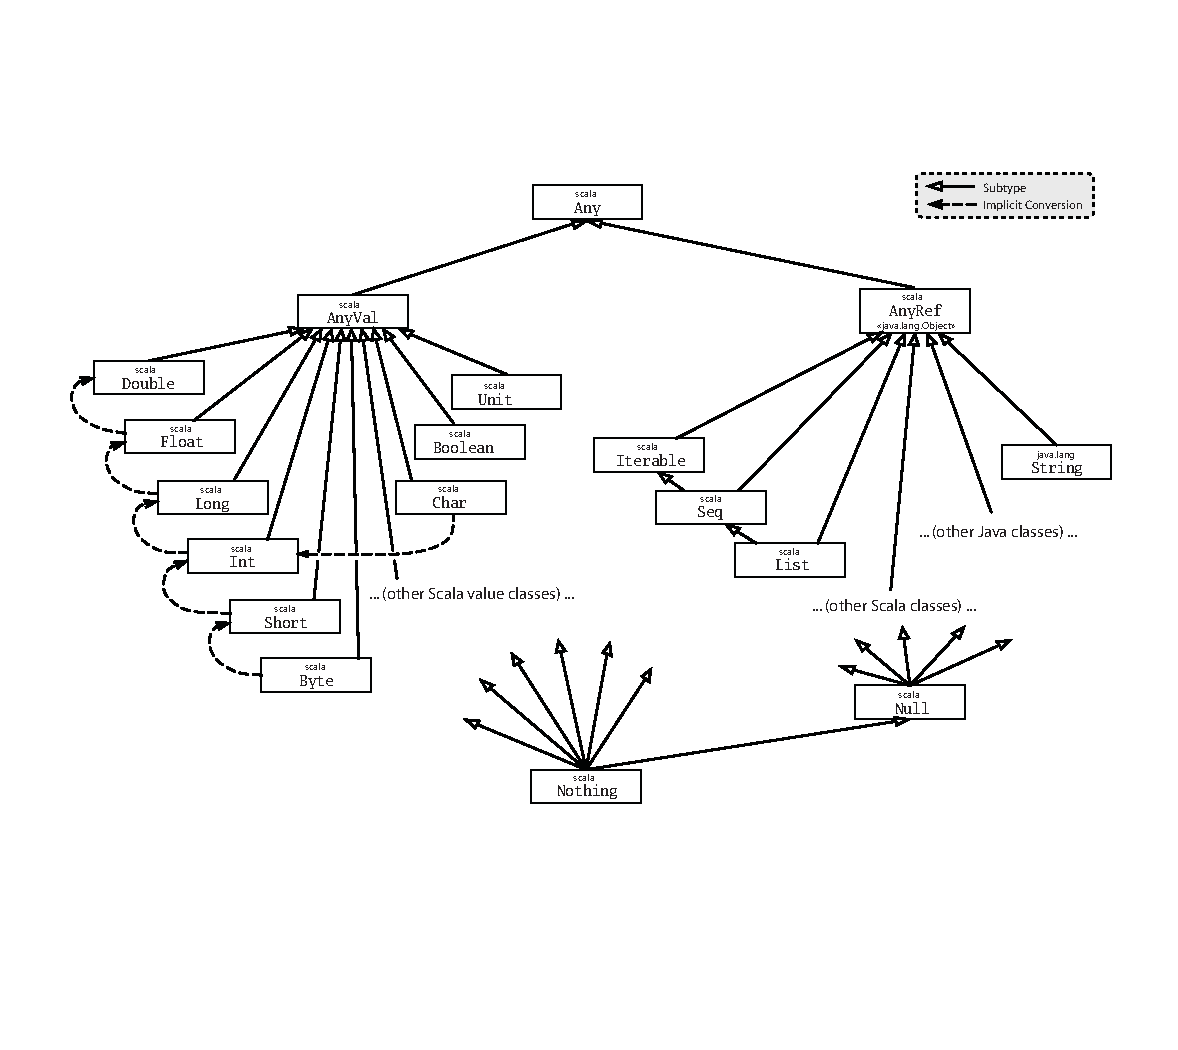
\includegraphics[width=1.05\textwidth,trim=12mm 0 0 0cm]{../img/hierarchy.pdf}

{\small \renewcommand{\arraystretch}{1.01}
\textbf{Number types}\\
\begin{tabular}{@{}l l @{\hspace{0.7em}}l @{\hspace{0.7em}}l @{}p{0.1em} | l l}
\textbf{name} & \textbf{\# bits} & \textbf{range} & \textbf{literal} &   & \multicolumn{2}{l}{\textbf{Methods on numbers}}\\ \cline{1-4}%\hline 
& & & &\\[-0.8em]
\texttt{Byte}   &  8  & $-2^7$ ... $2^7-1$  &\texttt{0.toByte} &  
& \code|x.abs| & \Comment{math.abs(x), absolute value}\\

\texttt{Short}  &  16 & $-2^{15}$ ... $2^{15}-1$ & \texttt{0.toShort}  &  
& \code|x.round| & \Comment{math.round(x), to nearest Long}\\

\texttt{Char}   &  16 & $0$ ... $2^{16}-1$ & \code|'0' '\u0030'| &  
& \code|x.floor| & \Comment{math.floor(x), cut decimals}\\

\texttt{Int}    &  32 & $-2^{31}$ ... $2^{31}-1$ & \texttt{0  0xF} & 
& \code|x.ceil| & \Comment{math.ceil(x), round up cut decimals}\\

\texttt{Long}   &  64 & $-2^{63}$ ... $2^{63}-1$ & \texttt{0L} & 
& \code|x max y| & \Comment{math.max(x, y), gives largest, also min}\\

\texttt{Float}  &  32 & ± $3.4 \cdot 10^{38}$  & \texttt{0F} &
& \code|x.toInt| & \Comment{also toByte, toChar, toDouble etc.}\\

\texttt{Double} &  64 & ± $1.8 \cdot 10^{308}$ & \texttt{0.0} & 
& \code|1 to 4| & \Comment{Range.inclusive(1, 4), contains 1,2,3,4}\\
 & & & & 
 & \code|0 until 4| & \Comment{Range(0, 4), contains 0,1,2,3}\\
 
 & & & & &  \code|Int.MinValue| & \Comment{least possible value of type Int}\\
 & & & & &  \code|Int.MaxValue| & \Comment{largest possible value of the Int}\\
  & & & & &   & \Comment{similar for all number types.}  \\
\end{tabular}
}


%%%%%%%%%%%%%%%%%%%%%%%%%%%%%%%%%%%%%%%%%%%%%%%%%%%%%%%%%%%%%%%%%%%%%%%%%%%%%
\Newline\vspace{-1em}\head{The Scala Standard Collection Library}
{
\small\renewcommand{\arraystretch}{1.1}
\begin{multicols}{2}
\texttt{scala.collection.}
\begin{tabular}{@{}l l l}
\texttt{immutable.} & \texttt{mutable.} & methods with good performance: \\
\hline
\texttt{Vector} & \texttt{ArrayBuffer} & \texttt{head tail apply~~+: :+}\\
\texttt{List} &  \texttt{ListBuffer} &  \texttt{head~~+:~~::}  \\
\texttt{Set} & \texttt{Set} & \texttt{contains~~+~~-}\\
\texttt{Map} & \texttt{Map} & \texttt{apply~~+~~-} \\
\end{tabular}

\vspace{0.2em}

\texttt{String} and \texttt{Array} are implicitly converted to \texttt{Seq}\\ making sequence methods work as for other sequences. \\

\vspace{0.5em} \textbf{Allocate array} of Int of size n: \code{new Array[Int](n)}

\columnbreak

\newcommand{\NodeSkip}{0.5cm}
\begin{center}
\tikzstyle{collectiontype}=[rectangle, draw=black,  thick, anchor=north, text width=1.7cm, rectangle split, rectangle split parts = 1]
\begin{tikzpicture}[node distance = \NodeSkip]
\node (Traversable) [collectiontype]  {\texttt{\centerline{Traversable}}};
\node (Iterable) [collectiontype, below = of Traversable]  {\texttt{\centerline{Iterable}}};        
\node (Seq) [collectiontype, below left = \NodeSkip and 0.05cm of Iterable,text width=1.0cm,]  {\texttt{\centerline{Seq}}}; 
\node (Set) [collectiontype, right = of Seq, text width=1.0cm,]  {\texttt{\centerline{Set}}};               
\node (Map) [collectiontype, right = of Set, text width=1.0cm,]  {\texttt{\centerline{Map}}};        
\node (Vector) [collectiontype, below left = \NodeSkip and -0.3cm of Seq, text width=1.0cm,]  {\texttt{\centerline{Vector}}};     
\node (List) [collectiontype, below right = \NodeSkip and -0.2cm of Seq, text width=1.0cm,]  {\texttt{\centerline{List}}};              
      
\draw[umlarrow] (Iterable.north) -- (Traversable.south);        
\draw[umlarrow] (Seq.north) -- (Iterable.south west);        
\draw[umlarrow] (Set.north) -- (Iterable.south);        
\draw[umlarrow] (Map.north) -- (Iterable.south east);        
\draw[umlarrow] (Vector.north) -- (Seq.south west);        
\draw[umlarrow] (List.north) -- (Seq.south east);        
\end{tikzpicture}
\end{center}
\end{multicols}
}

\vspace{-0.5em}{\small Concrete implementations of \textbf{Set} include HashSet, ListSet and BitSet; collection.\textbf{SortedSet} is implemented by TreeSet.\\
Concrete implementations of \textbf{Map} include HashMap and ListMap; collection.\textbf{SortedMap} is implemented by TreeMap.
}
%%%%%%%%%%%%%%%%%%%%%%%%%%%%%%%%%%%%%%%%%%%%%%%%%%%%%%%%%%%%%%%%%%%%%%%%%%%%%

%%%%%%%%%%%%%%%%%%%%%%%%%%%%%%%%%%%%%%%%%%%%%%%%%%%%%%%%%%%%%%%%%%%%%%%%%%%%%
\clearpage

\head{Methods in trait \texttt{Traversable[A]}}\Newline

{\small\renewcommand{\arraystretch}{1.2}
\begin{tabular}{@{}l p{3.5cm} p{6.8cm}}
\textbf{What} & \textbf{Usage} & \textbf{Explanation} f is a function, pf is a partial funct., p is a predicate.\\ \hline
Traverse: & \texttt{xs foreach f} & Executes f for every element of xs. Return type Unit.\\ \cline{1-3}

  Add: & \texttt{xs ++ ys} & A collection with xs followed by ys.\\\cline{1-3}
  
  Map: & \texttt{xs map f} & A collection formed by applying f to every element in xs.\\ \cline{2-3}
       & \texttt{xs flatMap f} & A collection obtained by applying f (which must return a collection) to all elements in xs and concatenating the results.\\ \cline{2-3}
       & \texttt{xs collect pf} & The collection obtained by applying the pf to every element in xs for which it is defined (undefined ignored).\\ \cline{1-3}

  Convert: & \texttt{toVector toList toSeq toBuffer toArray} & Converts a collection. Unchanged if the run-time type already matches the demanded type.\\ \cline{2-3}
   & \texttt{toSet} & Converts the collection to a set; duplicates removed.\\ \cline{2-3}
   & \texttt{toMap} & Converts a collection of key/value pairs to a map. \\ \cline{1-3}

  Copy: & \texttt{xs copyToBuffer buf } & Copies all elements of xs to buffer buf. Return type Unit.\\ \cline{2-3}
   & \texttt{xs copyToArray (arr, s, n)} & Copies at most n elements of the collection to array arr starting at index s (last two arguments are optional). Return type Unit.\\ \cline{1-3}

  Size info: & \texttt{xs.isEmpty} & Returns true if the collection xs is empty.\\ \cline{2-3}
   & \texttt{xs.nonEmpty} & Returns true if the collection xs has at least one element.\\ \cline{2-3}
   & \texttt{xs.size} & Returns an \texttt{Int} with the number of elements in xs.\\ \cline{1-3}
   

  Retrieval: & \texttt{xs.head xs.last} &  	The first/last element of xs (or some elem, if order undefined).\\ \cline{2-3}
      & \texttt{xs.headOption \newline xs.lastOption} & The first/last element of xs (or some element, if no order is defined) in an option value, or \texttt{None} if xs is empty.\\ \cline{2-3}
      & \texttt{xs find p} & An option with the first element satisfying p, or None.\\ \cline{1-3}


  Subparts: & \texttt{xs.tail xs.init} & The rest of the collection except xs.head or xs.last.\\ \cline{2-3}
      & \texttt{xs slice (from, to)} & The elements in from index \texttt{from} until (not including) \texttt{to}.\\ \cline{2-3}
      & \texttt{xs take n} & The first n elements (or some n elements, if order undefined).\\ \cline{2-3}
      & \texttt{xs drop n} & The rest of the collection except xs take n.\\ \cline{2-3}
      & \texttt{xs takeWhile p} & The longest prefix of elements all satisfying p.\\ \cline{2-3}
      & \texttt{xs dropWhile p} & Without the longest prefix of elements that all satisfy p.\\ \cline{2-3}
      & \texttt{xs filter p} & Those elements of xs that satisfy the predicate p. \\ \cline{2-3}
      & \texttt{xs filterNot p} & Those elements of xs that do not satisfy the predicate p.\\ \cline{2-3}
      & \texttt{xs splitAt n} &  	Split xs at n returning the pair (xs take n, xs drop n).\\ \cline{2-3}
      & \texttt{xs span p} & Split xs by p into the pair (xs takeWhile p, xs.dropWhile p).\\ \cline{2-3}
      & \texttt{xs partition p} & Split xs by p into the pair (xs filter p, xs.filterNot p)\\ \cline{2-3}
      & \texttt{xs groupBy f} & Partition xs into a map of collections according to f.\\ \cline{1-3}


  Conditions: & \texttt{xs forall p} & Returns true if p holds for all elements of xs.\\ \cline{2-3}
      & \texttt{xs exists p} & Returns true if p holds for some element of xs.\\ \cline{2-3}
      & \texttt{xs count p} & An \texttt{Int} with the number of elements in xs that satisfy p.\\ \cline{1-3}

  Folds: & \texttt{xs.foldLeft(z)(op) xs.foldRight(z)(op)} & Apply binary operation op between successive elements of xs, going left to right (or right to left) starting with z.\\ \cline{2-3}
      & \texttt{xs reduceLeft op \newline xs reduceRight op} & Similar to foldLeft/foldRight, but xs must be non-empty, starting with first element instead of z.\\ \cline{2-3}
      & \texttt{xs.sum xs.product xs.min xs.max} & Calculation of the sum/product/min/max of the elements of xs, which must be numeric.\\ \cline{1-3}
                              
   Make string: & \texttt{xs mkString (start, sep, end)} & A string with all elements of xs between separators sep enclosed in strings start and end; start, sep, end are all optional.\\ \cline{1-3}

   
\end{tabular}
}

\clearpage

\head{Methods in trait \texttt{Iterable[A]}}\Newline

{\small\renewcommand{\arraystretch}{1.1}
\begin{tabular}{@{}l p{3.4cm} p{6.8cm}}

\textbf{What} & \textbf{Usage} & \textbf{Explanation} \\ \hline

  Iterators: & \texttt{val it = xs.iterator} & An iterator \texttt{it} of type \texttt{Iterator} that yields each element one by one: \texttt{ while (it.hasNext) f(it.next)}\\   \cline{2-3}

   & \texttt{xs grouped size} & An iterator yielding fixed-sized chunks of this collection.\\\cline{2-3}
   & \texttt{xs sliding size} & An iterator yielding a sliding fixed-sized window of elements.\\\cline{1-3}

  Subparts: & \texttt{xs takeRight n \newline xs dropRight n} & Similar to \texttt{take} and \texttt{drop} in \texttt{Traversable} but takes/drops the last n elements (or any n elements if the order is undefined).\\   \cline{1-3}

  Zippers: & \texttt{xs zip ys} &  	An iterable of pairs of corresponding elements from xs and ys.\\   \cline{2-3}
   & \texttt{xs zipAll (ys, x, y)} & Similar to \texttt{zip}, but the shorter sequence is extended to match the longer one by appending elements x or y.\\\cline{2-3}
   & \texttt{xs.zipWithIndex} & An iterable of pairs of elements from xs with their indices.\\\cline{1-3}

  Compare: & \texttt{xs sameElements ys} & True if xs and ys contain the same elements in the same order.\\   \cline{1-3}

        
\end{tabular}
}  

\Newline
\head{Methods in trait \texttt{Seq[A]}}\Newline

{\small\renewcommand{\arraystretch}{1.1}
\begin{tabular}{@{}l p{3.75cm} p{6.8cm}}

%\textbf{What} & \textbf{Usage} & \textbf{Explanation} \texttt{f} is function, \texttt{pf} is partial funct., \texttt{p} is predicate.\\ \hline

  Indexing & \texttt{xs(i)  ~ xs apply i} & The element of xs at index i.\\   \cline{2-3}

   and size: & \texttt{xs.length} & Length of sequence. Same as \texttt{size} in \texttt{Traversable}.\\\cline{2-3}
   & \texttt{xs.indices} & Returns a \texttt{Range} extending from 0 to xs.length - 1.\\\cline{2-3}
   & \texttt{xs isDefinedAt i} & True if i is contained in xs.indices.\\\cline{2-3}
   & \texttt{xs lengthCompare n} & Returns -1 if xs is shorter than n, +1 if it is longer, else 0. \\\cline{1-3}

  
  Index & \texttt{xs indexOf x} & The index of the first element in xs equal to x.\\   \cline{2-3}
  search: & \texttt{xs lastIndexOf x} & The index of the last element in xs equal to x.\\\cline{2-3}
   & \texttt{xs indexOfSlice ys \newline xs lastIndexOfSlice ys} & The (last) index of xs such that successive elements starting from that index form the sequence ys.\\\cline{2-3}
   & \texttt{xs indexWhere p} & The index of the first element in xs that satisfies p.\\\cline{2-3}
   & \texttt{xs segmentLength (p, i)} & The length of the longest uninterrupted segment of elements in xs, starting with xs(i), that all satisfy the predicate p.\\\cline{2-3}
   & \texttt{xs prefixLength p} &  	Same as \texttt{ xs.segmentLength(p, 0)}\\\cline{1-3}


  Add: & {\texttt{x~+:~xs~~~~~xs~:+~x}}  & Prepend/Append x to xs. Colon on the collection side. \\   \cline{2-3}
   & \texttt{xs padTo (len, x)} & Append the value x to xs until length len is reached.\\\cline{1-3}
        

  Update: & \texttt{xs patch (i, ys, r)} &  A copy of xs with r elements of xs replaced by ys starting at i. \\   \cline{2-3}
   & \texttt{xs updated (i, x)} & A copy of xs with the element at index i replaced by x.\\\cline{2-3}
   & \texttt{xs(i) = x \newline xs.update(i, x)} & Only available for mutable sequences. Changes the element of xs at index i to x. Return type Unit.\\\cline{1-3}
        

  Sort: & \texttt{xs.sorted} & A new Seq[A] sorted using implicitly available ordering of A. \\   \cline{2-3}
   & \texttt{xs sortWith lt} &  	A new Seq[A] sorted using less than lt: (A, A) => Boolean.\\\cline{2-3}
By:  & \texttt{xs sortBy f} \newline \texttt{xs maxBy f} \texttt{~~xs minBy f}  &  	A new Seq[A] sorted/minimized/maximized by implicitly available ordering of B after applying f: A => B to each element.\\ \cline{1-3}
        

  Reverse: & \texttt{xs.reverse} & A new sequence with the elements of xs in reverse order. \\   \cline{2-3}
   & \texttt{xs.reverseIterator} & An iterator yielding all the elements of xs in reverse order.\\\cline{2-3}
   & \texttt{xs reverseMap f} & Similar to map in Traversable, but in reverse order.\\\cline{1-3}
        

  Tests: & \texttt{xs startsWith ys} & True if xs starts with sequence ys. \\   \cline{2-3}
   & \texttt{xs endsWith ys} & True if xs ends with sequence ys.\\\cline{2-3}
   & \texttt{xs contains x} & True if xs has an element equal to x.\\\cline{2-3}
   & \texttt{xs containsSlice ys} & True if xs has a contiguous subsequence equal to ys\\\cline{2-3}
   & \texttt{(xs corresponds ys)(p)} & True if corresponding elements satisfy the binary predicate p.\\\cline{1-3}
   
  Subparts: & \texttt{xs intersect ys} & The intersection of xs and ys, preserving element order.\\\cline{2-3}
   & \texttt{xs diff ys} & The difference of xs and ys, preserving element order.\\\cline{2-3}
   & \texttt{xs union ys} & Same as \texttt{xs ++ ys} in Traversable.\\\cline{2-3}
   & \texttt{xs.distinct} & A subsequence of xs that contains no duplicated element.\\\cline{1-3}
                   
       
        
\end{tabular}
}  

%\Newline
\vspace*{-0.5em}\head{Mutation methods in trait \texttt{mutable.Buffer[A]}, \texttt{ArrayBuffer[A]}, \texttt{ListBuffer[A]}    }\Newline
{\small\renewcommand{\arraystretch}{1.125}
\begin{tabular}{@{}p{5cm}  p{6.6cm}}
\texttt{xs(i) = x~~~~~xs.update(i, x)} & Replace element at index i with x. Return type Unit.\\   \cline{1-2}

\texttt{xs.insert(i, x)~~xs.remove(i)} & Insert x at index \texttt{i}. Remove element at i. Return type Unit.\\   \cline{1-2}

\texttt{xs.append(x)~~~~~xs~+=~x} & Insert x at end.  Return type Unit.\\   \cline{1-2}

\texttt{xs.prepend(x)~~~~x~+=:~xs} & Insert x in front.  Return type Unit.\\   \cline{1-2}

\texttt{xs -= x} & Remove first occurance of x (if exists). Returns xs itself. \\\cline{1-2}

\texttt{xs ++= ys} & Appends all elements in ys to xs and returns xs itself. \\\cline{1-2}

\end{tabular}
}

\Newline
\vspace*{-0.5em}\head{Methods in trait \texttt{Set[A]}}\Newline

{\small\renewcommand{\arraystretch}{1.125}
\begin{tabular}{@{}p{5cm}  p{6.6cm}}

%\textbf{Usage} & \textbf{Explanation} \\ \hline

\texttt{xs(x)~~~xs~apply~x} & True if x is a member of xs. Also: xs contains x\\   \cline{1-2}

\texttt{xs subsetOf ys} & True if ys is a subset of xs.\\\cline{1-2}

\texttt{xs~+~x~~~~~~~~~~xs - x} \newline \texttt{xs~+~(x,~y,~z)~~xs~-~(x,~y,~z)}& Returns a new set including/excluding elements. \newline Addition/subtraction can be applied to many arguments.\\   \cline{1-2}

\texttt{xs intersect ys} & A new set with elements in both xs and ys. Also: \texttt{\&} \\\cline{1-2}
\texttt{xs union ys} & A new set with elements in either xs or ys or both. Also: \texttt{|} \\\cline{1-2}
\texttt{xs diff ys} & A new set with elements in xs that are not in ys. Also: \texttt{\&\textasciitilde} \\\cline{1-2}
        
\end{tabular}
}  

\Newline
\vspace*{-0.5em}\head{Additional mutation methods in trait \texttt{mutable.Set[A]}}\Newline
{\small\renewcommand{\arraystretch}{1.125}
\begin{tabular}{@{}p{5cm}  p{6.6cm}}

\texttt{xs~+=~x~~~~~~~~~~xs~-=~x} & Returns the same set with included/excluded elements. \\   \cline{1-2}

\texttt{xs ++= ys} & Adds all elements in ys to set xs and returns xs itself. \\\cline{1-2}

\texttt{xs add x~~~xs remove x} & Adds/removes x to xs and returns true if x was in xs, else false. \\\cline{1-2}

%\texttt{xs retain p~~~xs.clear} & Keeps only elements that satisfy predicate p. Remove all.\\   \cline{1-2}
\texttt{xs(x) = b ~~~ xs.update(x, b)} & If b is true, adds x to xs, else removes x. Return type Unit.\\   \cline{1-2}
%\texttt{xs.clone} & Returns a new mutable set with the same elements as xs.\\   \cline{1-2}
        
\end{tabular}
}  

\Newline
\vspace*{-0.5em}\head{Methods in trait \texttt{Map[K, V]}}\Newline

{\small\renewcommand{\arraystretch}{1.125}
\begin{tabular}{@{}p{5.0cm}  p{6.6cm}}

\texttt{ms get k} & The value associated with key k an option, None if not found.\\   \cline{1-2}

\texttt{ms(k)~~~ms~apply~k} & The value associated with key k, or exception if not found.\\   \cline{1-2}

\texttt{ms getOrElse (k, d)} & The value associated with key k in map ms, or d if not found.\\   \cline{1-2}

\texttt{ms isDefinedAt k} & True if ms contains a mapping for key k. Also: ms.contains(k) \\   \cline{1-2}


\texttt{ms + (k -> v)  ~~ ms + ((k, v))} \newline \texttt{ms updated (k, v)} & The map containing all mappings of ms as well as the mapping k -> v from key k to value v. Also: ms + (k -> v, l -> w) \\   \cline{1-2}

\texttt{ms - k} & Excluding any mapping of key k. Also: ms - (k, l, m)\\   \cline{1-2}

\texttt{ms ++ ks ~~~~ ms {-}{-} ks} & The mappings of ms with the mappings of ks added/removed.\\   \cline{1-2}

\texttt{ms.keys~~ms.values~~ms.keySet} & An Iterable/Set containing each key/value in ms.\\   \cline{1-2}

\texttt{ms mapValues f} & A new Map obtained by applying f to values.\\   \cline{1-2}
        
\end{tabular}
}  


\Newline
\vspace*{-0.5em}\head{Additional mutation methods in trait \texttt{mutable.Map[K, V]}}\Newline

{\small\renewcommand{\arraystretch}{1.125}
\begin{tabular}{@{}p{5.0cm}  p{6.8cm}}

\texttt{ms(k) = v ~~ ms.update(k, v)} & Adds mapping k to v, overwriting any previous mapping of k.\\   \cline{1-2}

\texttt{ms += (k -> v) ~~~~ ms -= k} & Adds/Removes mappings. Also vid several arguments.\\   \cline{1-2}

\texttt{ms put (k, v) ~~ms remove k}& Adds/removes mapping; returns previous value of k as an option.\\   \cline{1-2}

%\texttt{ms retain p~~~ms.clear} & Keeps mappings with a key satisfying predicate p. Remove all.\\   \cline{1-2}

\texttt{ms transform f} & Transforms all associated values in map ms with function f.\\   \cline{1-2}

%\code|ms.clone| & Returns a new mutable map with the same mappings as ms.\\   \cline{1-2}
        
\end{tabular}
}  

\vspace{1.0em}\head{Factory examples:}\Newline

{\small%
\code{Vector(0, 0, 0)} \Comment{ same as } \code{Vector.fill(3)(0)} \\
\code{collection.mutable.Set.empty[Int]} \Comment{ same as } \code{collection.mutable.Set[Int]()}\\
\mbox{\code{Map("se" -> "Sweden","nk" -> "Norway")} \Comment{same as } 
\code{Map(("se","Sweden"),("nk","Norway"))}}\\
\code{Array.ofDim[Int](3,2)} \Comment{gives} \texttt{Array(Array(0, 0), Array(0, 0), Array(0, 0))} \Comment{same as} \texttt{Array.fill(3,2)(0)}; 
\texttt{ Vector.iterate(1.2, 3)(\_ + 0.5)} \Comment{gives} \texttt{Vector(1.2, 1.7, 2.2)}\\
\texttt{Vector.tabulate(3)("s" + \_) } \Comment{gives} \code{ Vector("s0", "s1", "s2")}
}




\clearpage

\Newline\head{Strings}\Newline


{\small\renewcommand{\arraystretch}{1.15}

Some methods below are from java.lang.String and some methods are implicitly added from StringOps, etc.\\ Strings are implictly treated as Seq[Char], so all Seq methods also work.

\vspace{0.5em}

\begin{tabular}{@{}l l}
\code|s(i)  s apply i   s.charAt(i)| & \Comment{Returns the character at index i.} \\
\code|s.capitalize| & \Comment{Returns this string with first character converted to upper case.} \\
\code|s.compareTo(t)| & \Comment{Returns x where x < 0 if s < t, x > 0 if s > t, x is 0 if s == t}\\
\code|s.compareToIgnoreCase(t)| & \Comment{Similar to compareTo but not sensitive to case.}\\
\code|s.endsWith(t)| & \Comment{True if string s ends with string t.} \\
\code|s.replaceAllLiterally(s1, s2)| & \Comment{Replace all occurances of s1 with s2 in s.} \\
\code|s.split(c)| & \Comment{Returns an array of strings split at every occurance of character c.} \\
\code|s.startsWith(t)| & \Comment{True if string s begins with string t.} \\
\code|s.stripMargin| & \Comment{Strips leading white space followed by | from each line in string.}\\
\code|s.substring(i)| & \Comment{Returns a substring of s with all charcters from index i.}\\
\code|s.substring(i, j)| & \Comment{Returns a substring of s from index i to index j-1.}\\
\code|s.toInt  s.toDouble  s.toFloat| & \Comment{Parses s as an Int or Double etc. May throw an exception.}\\
\code|42.toString   42.0.toString| & \Comment{Converts a number to a String.}\\
\code|s.toLowerCase| & \Comment{Converts all characters to lower case.}\\
\code|s.toUpperCase| & \Comment{Converts all characters to upper case.} \\
\code|s.trim| & \Comment{Removes leading and trailing white space.}\\
\end{tabular}
} 



\Newline

{\small\renewcommand{\arraystretch}{1.15}
\begin{tabular}{@{}p{0.7cm} l | r l}
\textbf{Escape} & \textbf{char} & \textbf{Special strings} & \\ 
\code|\n| & line break & \code|"hello\nworld\t!"| & \Comment{string including escape char for line break and tab}\\
\code|\t| & horisontal tab & \code|"""a "raw" string"""| & \Comment{can include quotes and span multiple lines}\\
\code|\"| & double quote '' & \code|s"x is $x"| & \Comment{\textbf{s interpolator} inserts values of existing names}\\
\code|\'| & single quote ' &  \code|s"x+1 is ${x+1}"|& \Comment{s interpolator evaluates expressions within}  \code|${}|\\
\code|\\| & backslash \textbackslash & \code|f"$x%5.2f"| & \Comment{format Double x to 2 decimals at least 5 chars wide}\\
\code|\u0041| &  unicode for A & \code|f"$y%5d"| & \Comment{format Int y right justified at least five chars wide}\\
\end{tabular}
} 



\Newline\head{scala.collection.JavaConverters}\Newline

{\small
Enable \code{.asJava} and \code{.asScala} conversions: \code{ import scala.collection.JavaConverters._ } 
\vspace{0.5em}

\begin{tabular}{@{}r c l}
\texttt{xs.asJava} on a \textbf{Scala} collection of type: & & \texttt{xs.asScala} on a \textbf{Java} collection of type: \\ 
\texttt{Iterator} &               $\longleftrightarrow$ & \texttt{java.util.Iterator} \\
\texttt{Iterable} &               $\longleftrightarrow$ & \texttt{java.lang.Iterable} \\
\texttt{Iterable} &               $\leftarrow$ & \texttt{java.util.Collection} \\
\texttt{mutable.Buffer} &         $\longleftrightarrow$  & \texttt{java.util.List} \\
\texttt{mutable.Set} &            $\longleftrightarrow$  & \texttt{java.util.Set} \\
\texttt{mutable.Map} &            $\longleftrightarrow$  & \texttt{java.util.Map} \\
\texttt{mutable.ConcurrentMap} &  $\longleftrightarrow$  & \texttt{java.util.concurrent.ConcurrentMap} \\\end{tabular}
}



\Newline\head{Reserved words}\Newline

{\small These 40 words and 10 symbols have special meaning and cannot be used as identifiers in Scala.}
 
\begin{Code}[morekeywords={macro,\_},otherkeywords={>,<-,\%,<,>:,@,:,=,\#}]
abstract case catch class def do else extends false final finally for 
forSome if  implicit import lazy macro match new null object override 
package private protected return sealed super this throw trait try true 
type val var while with yield   _   :   =   =>   <-   <:   <%   >:   #   @ 
\end{Code}


%%%************************************************************************************
%%%*************************** JAVA STARTS HERE ***************************************
%%%************************************************************************************

%%%%% TODO: Translate to English

\clearpage\renewcommand{\arraystretch}{0.91}
\setcounter{page}{1}
\renewcommand{\LangColor}{blue}
\LangMarker{Java}{3.5cm}{4}

\LangTitle{Java snabbreferens  @ LTH}
\vspace{1em}
%% CHANGED BY BJORNR:
{\small Vertikalstreck \Or~används mellan olika alternativ. Parenteser \RepL \RepR används för att gruppera en mängd alternativ. Hakparenteser \OptL \OptR markerar valfria delar. En sats betecknas \jcode{stmt} medan \jcode{x}, \jcode{i}, \jcode{s}, \jcode{ch} är variabler, \jcode{expr} är ett uttryck, \jcode{cond} är ett logiskt uttryck. Med \verb|...| avses valfri, extra kod.}

%{\small Tecknet ~|~ står för ''eller''. Vanliga parenteser~(~)~används för att gruppera alternativ. Med~[~]~markeras sådant som inte alltid finns med. Med \jcode{stmt} avses en sats, \jcode{x}, \jcode{i}, \jcode{s}, \jcode{ch} är variabler, \jcode{expr} är ett uttryck, \jcode{cond} är ett logiskt uttryck.}


\Newline
\head{Satser}\Newline
{\small
\begin{tabular}{@{}l l l}
Block   & \jcode|{stmt1; stmt2; ...}| &  fungerar ''utifrån'' som \textbf{en} sats \secend

Tilldelning & \verb|x = expr;|                 &  variabeln och uttrycket av kompatibel typ \secend

Förkortade       & \verb|x += expr; |                &  x = x + expr; även --=, *=, /= \\
                 & \verb|x++;  |                     &  x = x + 1; även x\hspace{0.5mm}-- -- \secend

if-sats          & \verb|if (cond) {stmt; ...}|      &  utförs om cond är true \\
                 & \OptL \verb|else { stmt; ...}| \OptR&  utförs om false \secend

switch-sats      & \verb|switch (expr) {|         &  expr är ett heltalsuttryck \\ 
                 & \verb|    case A: stmt1; break;|  &  utförs om expr $=$ A (A konstant) \\
                 & \verb|    ...|                 & ''faller igenom'' om break saknas\\
                 & \verb|    default: stmtN; break;| &  sats efter default: utförs om inget case passar\\
                 & \verb|}|                   & \secend

for-sats         & \verb|for (int i = a; i < b; i++) {| & satserna görs för i = a, a+1, \ldots, b-1\\
                 & \verb|    stmt; ...|  & Görs ingen gång om a >= b \\
                 & \verb|}  |         &  i++ kan ersättas med i = i + step \secend

%ADDED BY BJORNR                 
for-each-sats    & \verb|for (int x: xs) {|   & xs är en samling, här med heltal  \secend
                 & \verb|    stmt; ...|  & x blir ett element i taget ur xs\\
                 & \verb|}  |         &  fungerar även med array \secend

while-sats       & \verb|while (cond) {stmt; ...}|          & utförs så länge cond är true \secend

do-while-sats    & \verb|do {|                     & \\
                 & \verb|    stmt; ...|         &  utförs minst en gång, \\
                 & \verb|} while (cond);|          &  så länge cond är true \secend

return-sats      & \verb|return expr;|        &  returnerar funktionsresultat
\end{tabular}
}

\Newline\head{Uttryck}
\begin{etab}
Aritmetiskt uttryck & (x + 2) * i / 2 + i \% 2   &  för heltal är / heltalsdivision, \% ''rest''   \secend


Objektuttryck     & \mc{new Classname(\ldots) \Or ref-var \Or null \Or function-call \Or this \Or super} \secend

Logiskt uttryck   & \mc{! cond \Or  cond \&\& cond \Or  cond || cond \Or  relationsuttryck \Or true \Or  false} \subsecend

Relationsuttryck  & expr \RepL < \Or <= \Or == \Or >= \Or > \Or != \RepR expr & för objektuttryck bara == och !=, också typtest med expr instanceof Classname \subsecend

Funktionsanrop    & obj-expr.method(\ldots)    &  anropa ''vanlig metod'' (utför operation) \\
                  & Classname.method(\ldots)   &  anropa statisk metod \secend

Array             & new int[size]              &  skapar int-array med size element \\
                  & vname[i]                   &  elementet med index i, 0..length$-1$\\
                  & vname.length               &  antalet element \secend

%ADDED BY SANDRA:
Matris		      & new int[r][c]			   & //Skapar matris med r rader och c kolonner\\
   				& m.length			   & //Ger matrisens längd (d.v.s. antalet rader) \\
 				  & m[i].length			   & //Ger antalet element (längden) på raden i  \secend

Typkonvertering   & (newtype) expr             &  konverterar expr till typen newtype \\
                  & (int) real-expr            &  -- avkortar genom att stryka decimaler \\
                  & (Square) aShape            &  -- ger ClassCastException om aShape inte \\
                  &                            &  är ett Square-objekt
\end{etab}


\clearpage
\head{Deklarationer}
\begin{etab}
Allmänt           & \mc{\OptL<protection> \OptR  \OptL static \OptR \OptL final \OptR <type> name1, name2, \ldots;} \secend

<type>            & \mc{byte \Or short \Or int \Or long \Or float \Or double \Or boolean \Or char \Or Classname} \secend

<protection>      & public \Or private \Or protected &  för attribut och metoder i klasser \\
                  &                             &  (paketskydd om inget anges) \secend

Startvärde        & int x = 5;                  &  startvärde bör alltid anges \secend

Konstant          & final int N = 20;           &  konstantnamn med stora bokstäver \secend

Array             & <type>[\hspace{0.4mm}] vname = new <type>[10]; &  deklarerar och skapar array \secend

%ADDED BY SANDRA
Matris            & <type>[\hspace{0.4mm}][\hspace{0.4mm}] m = new <type>[4][5]; & // deklarerar och skapar 4x5 matrisen m \secend

\end{etab}


\head{Klasser}
\begin{etab}
Deklaration       & \OptL public\OptR \OptL abstract \OptR class Classname & \\
                  & \mc{\ind \OptL extends Classname1\OptR \OptL implements Interface1, Interface2, \ldots\OptR $\{$} \\
                  & \ind <deklaration av attribut> & \\
                  & \ind <deklaration av konstruktorer> & \\
                  & \ind <deklaration av metoder> & \\
                  & $\}$                          & \secend

Attribut          & \mc{Som vanliga deklarationer. Attribut får implicita startvärden, 0, 0.0, false, null.} \secend

Konstruktor       & <prot> Classname(param, \ldots) $\{$ &  Parametrarna är de parametrar som ges vid \\
                  & \ind stmt; \ldots              &  new Classname(\ldots). Satserna ska ge \\ 
                  & $\}$                           &  attributen startvärden \secend

Metod             & <prot> <type> name(param, \ldots) $\{$ &  om typen inte är void måste en return-\\
                  & \ind stmt; \ldots              &  sats exekveras i metoden \\
                  & $\}$                           & \secend
                  
Huvudprogram      & \mc{public static void main(String[\hspace{0.5mm}] args) $\{$ \ldots $\}$} \secend

Abstrakt metod    & \mc{Som vanlig metod, men abstract före typnamnet och $\{\ldots\}$ ersätts med semikolon. Metoden måste implementeras i subklasserna.}
\end{etab}

\head{Standardklasser, java.lang, behöver inte importeras}
\begin{etab}
Object            & \mc{Superklass till alla klasser.} \subsecend
                  & boolean equals(Object other);   &  ger true om objektet är lika med other \\
                  & int hashCode();                 &  ger objektets hashkod \\
                  & String toString();              &  ger en läsbar representation av objektet \secend
                  
Math              & \mc{Statiska konstanter Math.PI och Math.E. Metoderna är statiska (anropas med t~ex Math.round(x)):} \subsecend
                  & long round(double x);           &  avrundning, även float $\rightarrow$ int \\
                  & int abs(int x);                 &  $|x|$, även double, \ldots \\
                  & double hypot(double x, double y); &  $\sqrt{x^2+y^2}$ \\
                  & double sin(double x);           &  $\sin x$, liknande: cos, tan, asin, acos, atan \\
                  & double exp(double x);           &  $e^x$ \\
                  & double pow(double x, double y); &  $x^y$ \\
                  & double log(double x);           &  $\ln x$ \\
                  & double sqrt(double x);          &  $\sqrt{x}$ \\
                  & double toRadians(double deg);   &  $\mathit{deg} \cdot \pi / 180$ \secend

System            & void System.out.print(String s); &  skriv ut strängen s \\
                  & void System.out.println(String s); &  som print men avsluta med ny rad \\
                  & void System.exit(int status);   &  avsluta exekveringen, status != 0 om fel \\
                  & \mc{Parametern till print och println kan vara av godtycklig typ: int, double, \ldots} \secend
\end{etab}
\clearpage
\begin{etab}
Wrapperklasser     & \mc{För varje datatyp finns en wrapperklass: char $\rightarrow$ Character, int $\rightarrow$ Integer, double $\rightarrow$ Double, \ldots\ 
Statiska konstanter MIN\_VALUE och MAX\_VALUE i klassen Integer ger minsta respektive största heltalsvärde. För klassen Double ger MIN\_VALUE minsta flyttalet som är större än noll.\\
Exempel med klassen Integer:} \subsecend
                  & Integer(int value);             &  skapar ett objekt som innehåller value \\
                  & int intValue();                 &  tar reda på värdet \secend

String            & \mc{Teckensträngar där tecknen inte kan ändras. ''asdf'' är ett String-objekt. s1 + s2 för att konkatenera två strängar. StringIndexOutOfBoundsException om någon position är fel.} \subsecend
                  & int length();                   &  antalet tecken \\
                  & char charAt(int i);             &  tecknet på plats i, 0..length()$-1$ \\
                  & boolean equals(String s);       &  jämför innehållet (s1 == s2 fungerar inte) \\
                  & int compareTo(String s);        &  < 0 om mindre, = 0 om lika, > 0 om större \\
                  & int indexOf(char ch);           &  index för ch, $-1$ om inte finns \\
                  & int indexOf(char ch, int from); &  som indexOf men börjar leta på plats from \\
                  & String substring(int first, int last); &  kopia av tecknen first..last$-1$ \\
                  & String[\hspace{0.5mm}] split(String delim); &  ger array med ''ord'' (ord är följder av \\
                  &                                 &  tecken åtskilda med tecknen i delim) \secend

                  & \mc{Konvertering mellan standardtyp och String (exempel med int, liknande för andra typer):} \\%\subsecend
                  & String.valueOf(int x);          &  x = 1234 $\rightarrow$ ''1234'' \\ 
                  & Integer.parseInt(String s);     &  s = ''1234'' $\rightarrow$ 1234, NumberFormat- \\
                  &                                 &  Exception om s innehåller felaktiga tecken \secend

StringBuilder     & \mc{Modifierbara teckensträngar. length och charAt som String, plus:} \subsecend
                  & StringBuilder(String s);        &  StringBuilder med samma innehåll som s \\
                  & void setCharAt(int i, char ch); &  ändrar tecknet på plats i till ch \\
                  & StringBuilder append(String s); &  lägger till s, även andra typer: int, char, \ldots \\
                  & StringBuilder insert(int i, String s); &  lägger in s med början på plats i \\
                  & StringBuilder deleteCharAt(int i); &  tar bort tecknet på plats i \\ 
                  & String toString();              &  skapar kopia som String-objekt
\end{etab}

\head{Standardklasser, import java.util.Classname}
\begin{etab}
List              & \mc{List<E> är ett gränssnitt som beskriver listor med objekt av parameterklassen E. Man kan lägga in värden av standardtyperna genom att kapsla in dem, till exempel int i Integer-objekt. Gränssnittet implementeras av klasserna ArrayList<E> och LinkedList<E>, som har samma operationer. Man ska inte använda operationerna som har en position som parameter på en LinkedList (i stället en iterator). IndexOutOfBoundsException om någon position är fel.} \subsecend
                  & \mc{För att operationerna contains, indexOf och remove(Object) ska fungera måste klassen E överskugga funktionen equals(Object). Integer och de andra wrapperklasserna gör det.} \subsecend
ArrayList         & ArrayList<E>();                 &  skapar tom lista \\ 
LinkedList        & LinkedList<E>();                &  skapar tom lista \\ 
                  & int size();                     &  antalet element \\
                  & boolean isEmpty();              &  ger true om listan är tom \\
                  & E get(int i);                   &  tar reda på elementet på plats i \\
                  & int indexOf(Object obj);        &  index för obj, $-1$ om inte finns \\
                  & boolean contains(Object obj);   &  ger true om obj finns i listan \\

                  & void add(E obj);                &  lägger in obj sist, efter existerande element \\
                  & void add(int i, E obj);         &  lägger in obj på plats i (efterföljande \\
                  &                                 &  element flyttas) \\
                  & E set(int i, E obj);            &  ersätter elementet på plats i med obj \\
                  & E remove(int i);                &  tar bort elementet på plats i (efter- \\
                  &                                 &  följande element flyttas) \\
                  & boolean remove(Object obj);     &  tar bort objektet obj, om det finns \\
                  & void clear();                   &  tar bort alla element i listan \secend

\end{etab}
\secend
\begin{etab}

Random            & Random();                       &  skapar ''slumpmässig'' slumptalsgenerator \\
                  & Random(long seed);              &  -- med bestämt slumptalsfrö \\
                  & int nextInt(int n);             &  heltal i intervallet [0, n) \\
                  & double nextDouble();            &  double-tal i intervallet [0.0, 1.0) \secend

Scanner           & Scanner(File f);                &  läser från filen f, ofta System.in \\
                  & Scanner(String s);              &  läser från strängen s \\
                  & String next();                  &  läser nästa sträng fram till whitespace \\
                  & boolean hasNext();              &  ger true om det finns mer att läsa \\
                  & int nextInt();                  &  nästa heltal; också nextDouble(), \ldots \\
                  & boolean hasNextInt();           &  också hasNextDouble(), \ldots \\
                  & String nextLine();              &  läser resten av raden
\end{etab}



\head{Filer, import java.io.File/FileNotFoundException/PrintWriter}
\begin{etab}
Läsa från fil     & \mc{Skapa en Scanner med new Scanner(new File(filename)). Ger File\-NotFoundException om filen inte finns. Sedan läser man ''som vanligt'' från scannern (nextInt och liknande).} \subsecend
                  
Skriva till fil   & \mc{Skapa en PrintWriter med new PrintWriter(new File(filename)). Ger FileNotFoundException om filen inte kan skapas. Sedan skriver man ''som vanligt'' på PrintWriter-objektet (println och liknande).}\subsecend

Fånga undantag    & \mc{Så här gör man för att fånga FileNotFoundException:\\[1mm]
\ind Scanner scan = null;\\
\ind try $\{$\\
\ind \ind scan = new Scanner(new File("indata.txt"));\\
\ind $\}$ catch (FileNotFoundException e) $\{$\\
\ind \ind \ldots\ ta hand om felet\\
\ind $\}$}
\end{etab}


\head{Specialtecken}
\begin{etab}
                  & \mc{Några tecken måste skrivas på ett speciellt sätt när de används i teckenkonstanter:}\subsecend

& \textbackslash{}n & ny rad, radframmatningstecken\\
& \textbackslash{}t & ny kolumn, tabulatortecken (eng. tab)\\
& \textbackslash{}\textbackslash{} & bakåtsnedstreck: \textbackslash{} (eng. {\em backslash})\\
& \textbackslash{}'' & citationstecken: ''\\
& \textbackslash{}' & apostrof: '\\

\end{etab}

\head{Reserverade ord}\Newline

{\small Nedan 50 ord kan ej användas som identifierare i Java. Orden \jcode{goto} och \jcode{const} är reserverade men används ej.}
 
\begin{Code}[language=Java,morekeywords={assert, enum, strictfp}]
abstract assert boolean break byte case catch char class const 
continue default do double else enum extends final finally float for 
goto if implements import instanceof int interface long native new 
package private protected public return short static strictfp super 
switch synchronized this throw throws transient try void volatile while
\end{Code}


\end{document}